\section{Conclusion}
\label{sec:conclusion}

Summing up, in this laboratory assignment (T2) we have made both theoretical analysis as well as simulations of several different but similar and correlated circuits. \par
The results obtained in both analysis were either put in a table or plotted in order to make comparations between the theoretical and simulation analysis.
Up untill the simulation's question 4, the results are either the exact same or have very little differences on the last decimal places and so they are negligible, the explanation for this is that we studied a very simple circuit containing only linear components. If the components used were more complex, the case would not be the same and we could detect real differences between the values calculated and simulated. \par
Comparing figure 17 and figure 18, the theoretical value is based on a simplification when the circuit contribuition is resumed to $R_{eq}$ and, the NGspice result is based on all the actual contributions of the circuit. Thus in the figure 18 the signal is going to be a perfect sinusoidal signal while the figure 17 displays an imperfect signal. \par
Lastly, for the same reasons of figure 17 and 18, there are little differences between plots in both figures. \par
That being said we would like to end this report by presenting both the theoretical and simulation results side by side in order to easily compare the results. \par

\begin{figure}[H]
    \minipage{0.50\textwidth}
      \centering
      \begin{tabular}{ | c | c | }
      \hline    
      {\bf Name} & {\bf Value [A or V]} \\ \hline
      $V_1$ & 5.025226e+00 \\ \hline 
$V_2$ & 4.724476e+00 \\ \hline 
$V_3$ & 4.104661e+00 \\ \hline 
$V_5$ & 4.765766e+00 \\ \hline 
$V_6$ & 5.702373e+00 \\ \hline 
$V_7$ & -1.847813e+00 \\ \hline 
$V_8$ & -2.790649e+00 \\ \hline 
$I_1$ & -2.870701e-04 \\ \hline 
$I_2$ & -3.006765e-04 \\ \hline 
$I_3$ & 1.360640e-05 \\ \hline 
$I_4$ & 1.190255e-03 \\ \hline 
$I_5$ & 3.006765e-04 \\ \hline 
$I_6$ & 9.031846e-04 \\ \hline 
$I_7$ & 9.031846e-04 \\ \hline 
$I_s$ & -2.870701e-04 \\ \hline 
$I_d$ & 9.031846e-04 \\ \hline 
$I_b$ & -3.006765e-04 \\ \hline 
$I_c$ & -2.168404e-19 \\ 

      \hline
      \end{tabular}
      \caption{Theoretical Question 1}
    \endminipage\hfill
    \minipage{0.50\textwidth}
      \centering
      \begin{tabular}{ | c | c | }
      \hline    
      {\bf Name} & {\bf Value [A or V]} \\ \hline
      @c0[i] & 0.000000e+00\\ \hline
@g0[i] & -3.00677e-04\\ \hline
@r1[i] & 2.870701e-04\\ \hline
@r2[i] & -3.00677e-04\\ \hline
@r3[i] & -1.36064e-05\\ \hline
@r4[i] & 1.190255e-03\\ \hline
@r5[i] & -3.00677e-04\\ \hline
@r6[i] & 9.031846e-04\\ \hline
@r7[i] & 9.031846e-04\\ \hline
n1 & 5.025226e+00\\ \hline
n2 & 4.724476e+00\\ \hline
n3 & 4.104661e+00\\ \hline
n5 & 4.765766e+00\\ \hline
n6 & 5.702373e+00\\ \hline
n7 & -1.84781e+00\\ \hline
n8 & -2.79065e+00\\ \hline
n9 & -2.79065e+00\\ \hline

      \end{tabular}
      \caption{Simulation Question 1}
    \endminipage\hfill
\end{figure}

\begin{figure}[H]
    \minipage{0.50\textwidth}
      \centering
      \begin{tabular}{ | c | c | }
      \hline    
      {\bf Name} & {\bf Value [A or V]} \\ \hline
      $V_x$ & 8.493021e+00 \\ \hline 
$V_1$ & 0.000000e+00 \\ \hline 
$V_2$ & 0.000000e+00 \\ \hline 
$V_3$ & -0.000000e+00 \\ \hline 
$V_5$ & 0.000000e+00 \\ \hline 
$V_6$ & 8.493021e+00 \\ \hline 
$V_7$ & 0.000000e+00 \\ \hline 
$V_8$ & 0.000000e+00 \\ \hline 
$I_1$ & 0.000000e+00 \\ \hline 
$I_2$ & 0.000000e+00 \\ \hline 
$I_3$ & 0.000000e+00 \\ \hline 
$I_4$ & 0.000000e+00 \\ \hline 
$I_5$ & 2.726493e-03 \\ \hline 
$I_6$ & -0.000000e+00 \\ \hline 
$I_7$ & -0.000000e+00 \\ \hline 
$I_s$ & 0.000000e+00 \\ \hline 
$I_d$ & -0.000000e+00 \\ \hline 
$I_b$ & 0.000000e+00 \\ \hline 
$I_x$ & 2.726493e-03 \\ \hline 
$Req (kOhm)$ & 3.114999e+00 \\ \hline 
$tau (ms)$ & 3.145605e+00 \\ 

      \hline
      \end{tabular}
      \caption{Theoretical Question 2}
    \endminipage\hfill
    \minipage{0.50\textwidth}
      \centering
      \begin{tabular}{ | c | c | }
      \hline    
      {\bf Name} & {\bf Value [A or V]} \\ \hline
      @g0[i] & 0.000000e+00\\ \hline
@r1[i] & 0.000000e+00\\ \hline
@r2[i] & 0.000000e+00\\ \hline
@r3[i] & 0.000000e+00\\ \hline
@r4[i] & 0.000000e+00\\ \hline
@r5[i] & 2.726492e-03\\ \hline
@r6[i] & 0.000000e+00\\ \hline
@r7[i] & 0.000000e+00\\ \hline
n1 & 0.000000e+00\\ \hline
n2 & 0.000000e+00\\ \hline
n3 & 0.000000e+00\\ \hline
n5 & 0.000000e+00\\ \hline
n6 & -8.49302e+00\\ \hline
n7 & 0.000000e+00\\ \hline
n8 & 0.000000e+00\\ \hline
n9 & 0.000000e+00\\ \hline

      \end{tabular}
      \caption{Simulation Question 2}
    \endminipage\hfill
\end{figure}

\begin{figure}[H]
    \minipage{0.45\textwidth}
      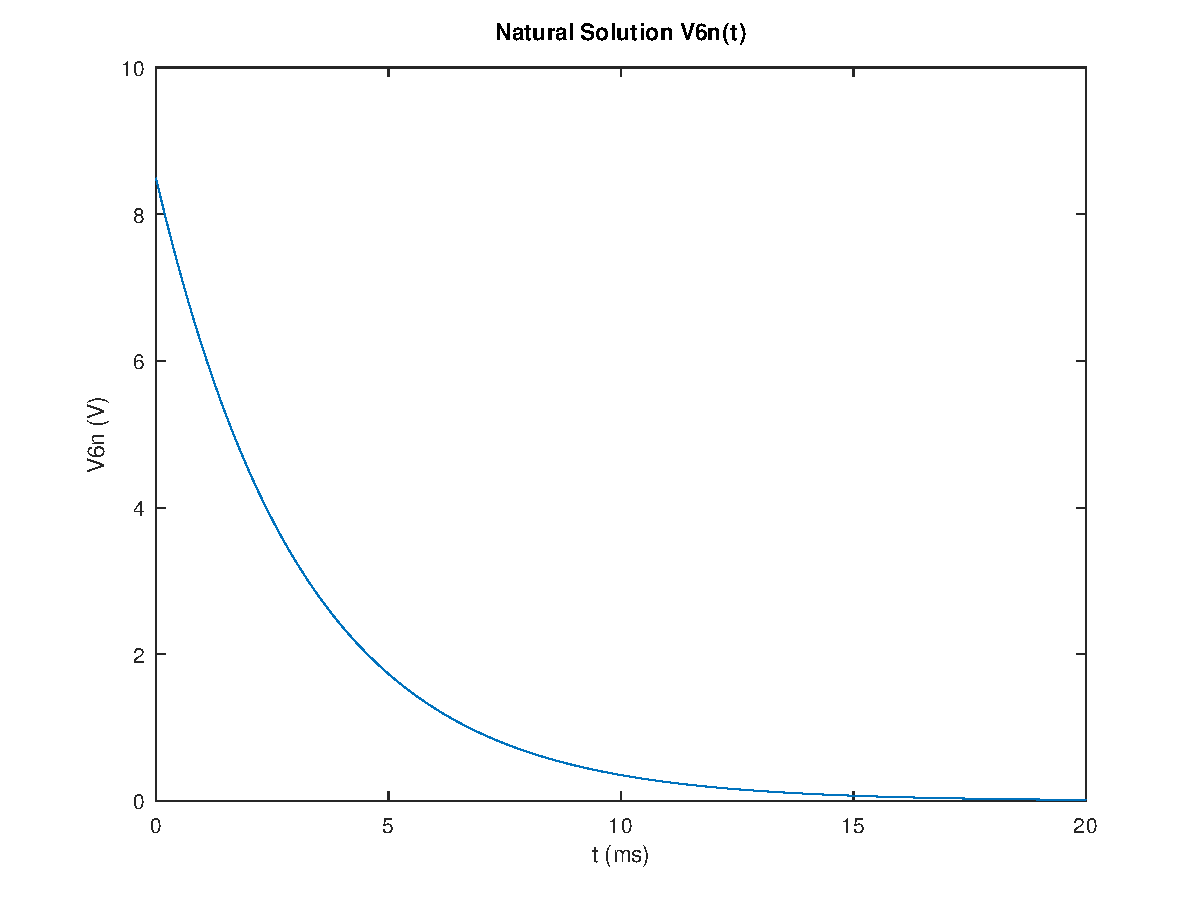
\includegraphics[width=\linewidth]{../mat/alinea3.pdf}
      \caption{Theoretical Question 3}
    \endminipage\hfill
    \minipage{0.45\textwidth}
      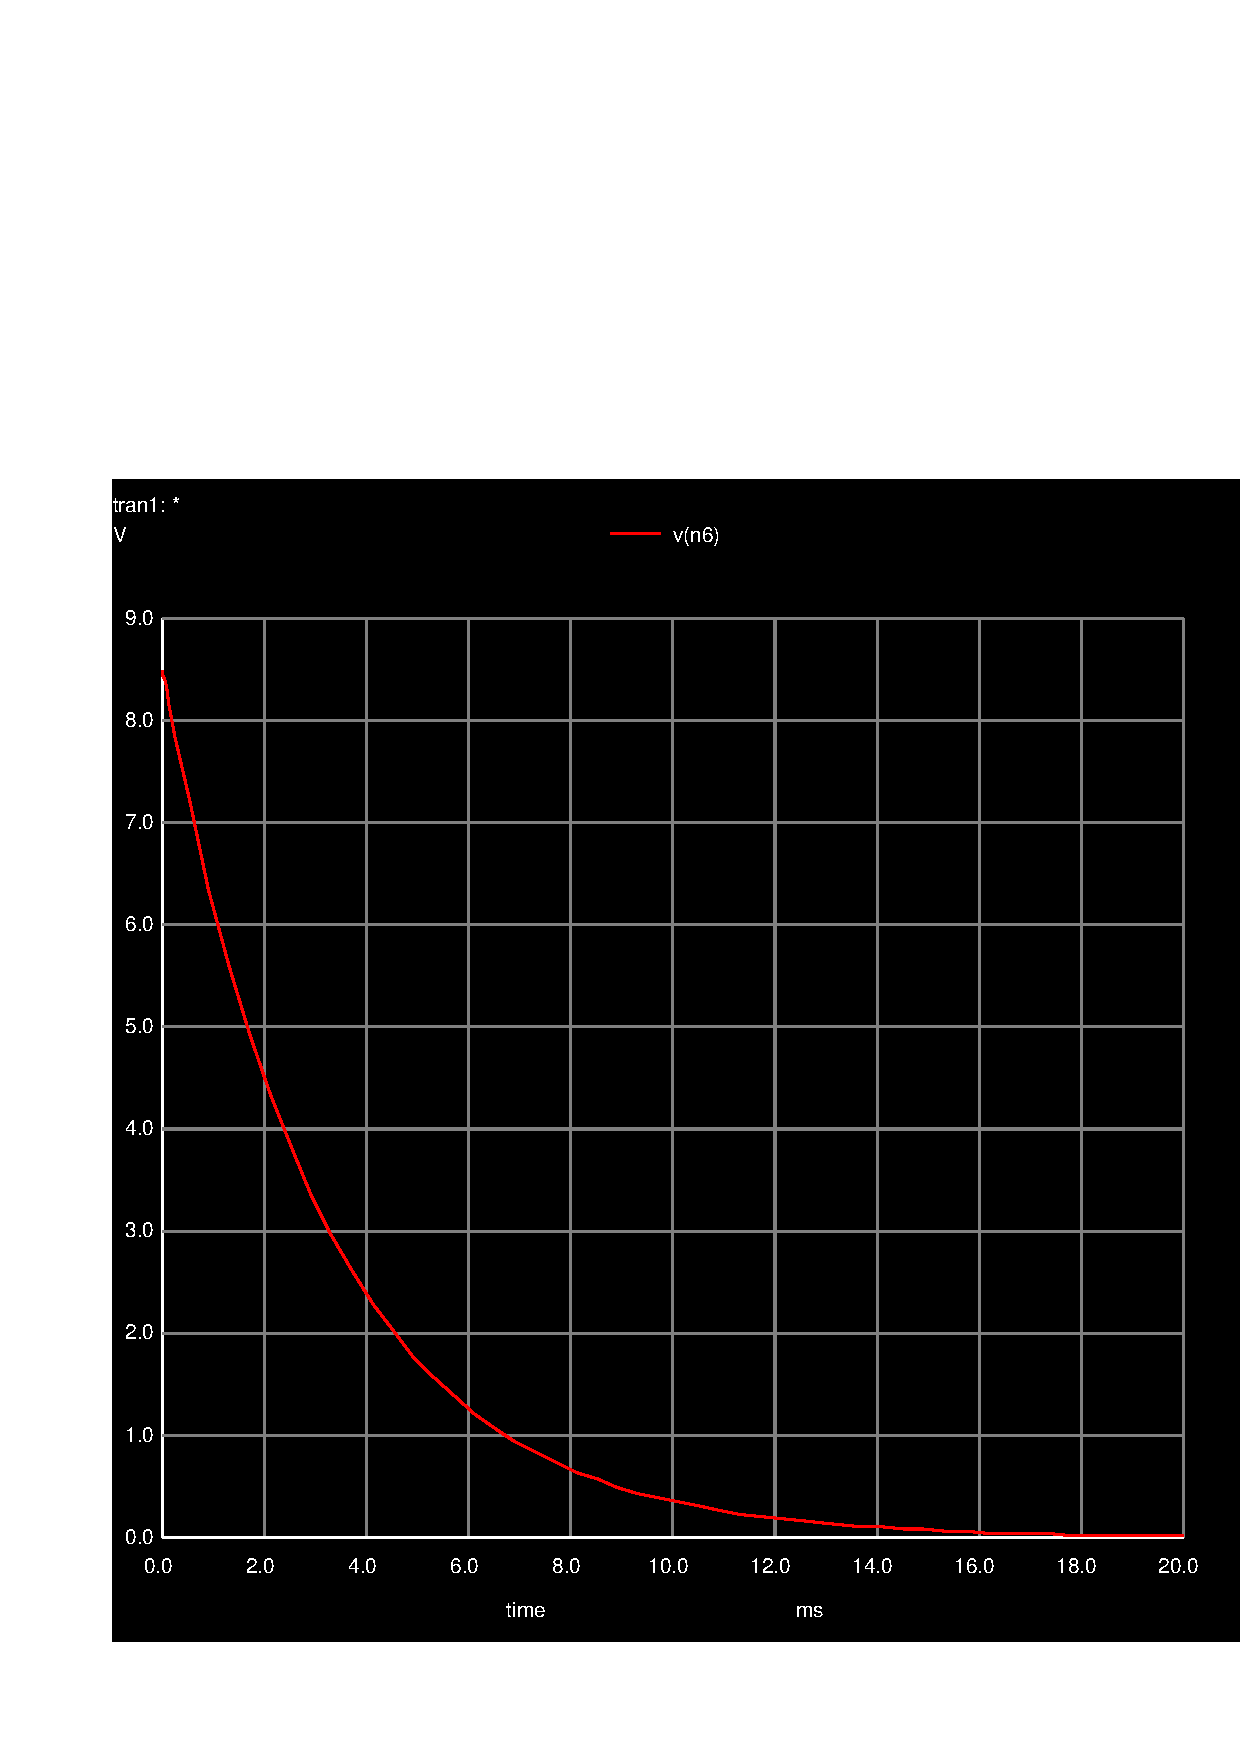
\includegraphics[width=\linewidth]{../sim/transient3.pdf}
      \caption{Simulation Question 3}
    \endminipage\hfill
\end{figure}

\begin{figure}[H]
    \minipage{0.45\textwidth}
      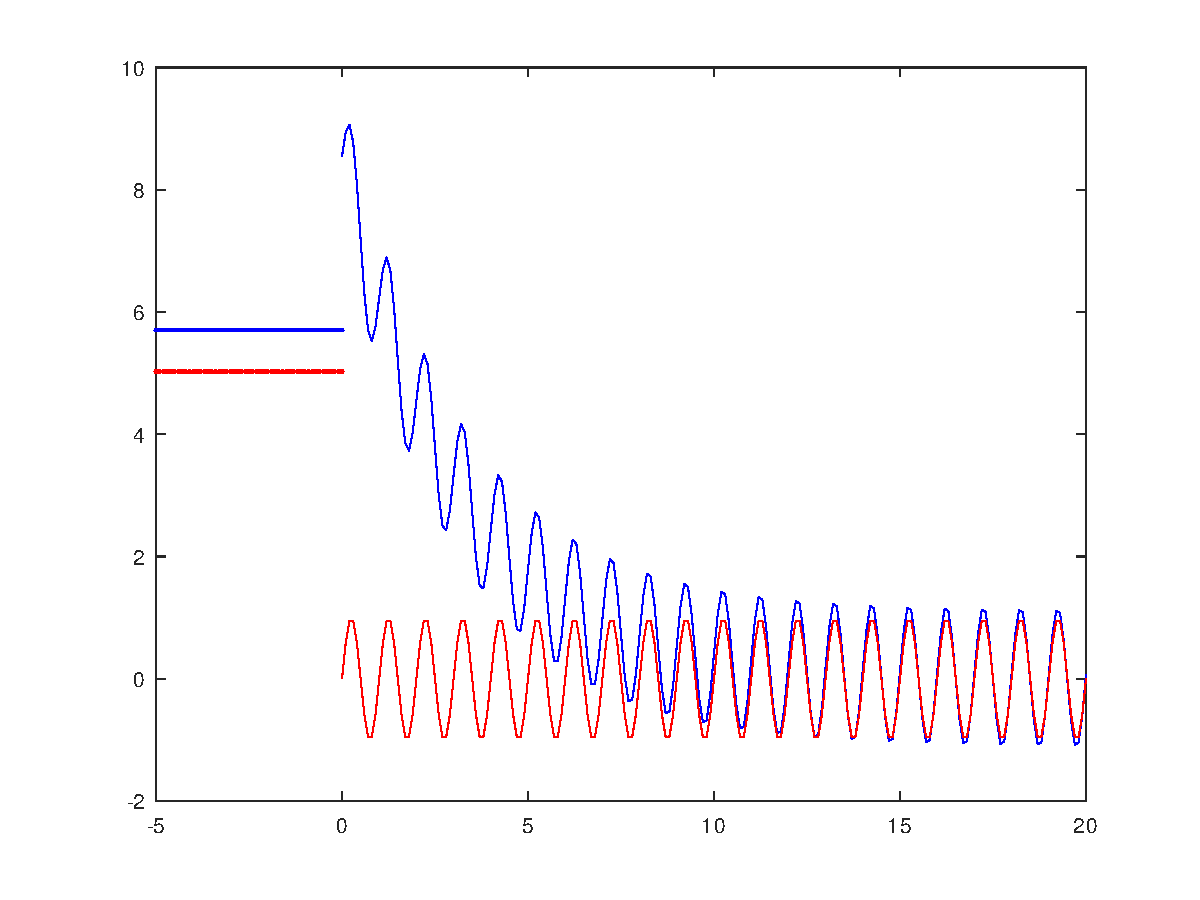
\includegraphics[width=\linewidth]{../mat/alinea5.pdf}
      \caption{Theoretical Question 5}
    \endminipage\hfill
    \minipage{0.45\textwidth}
      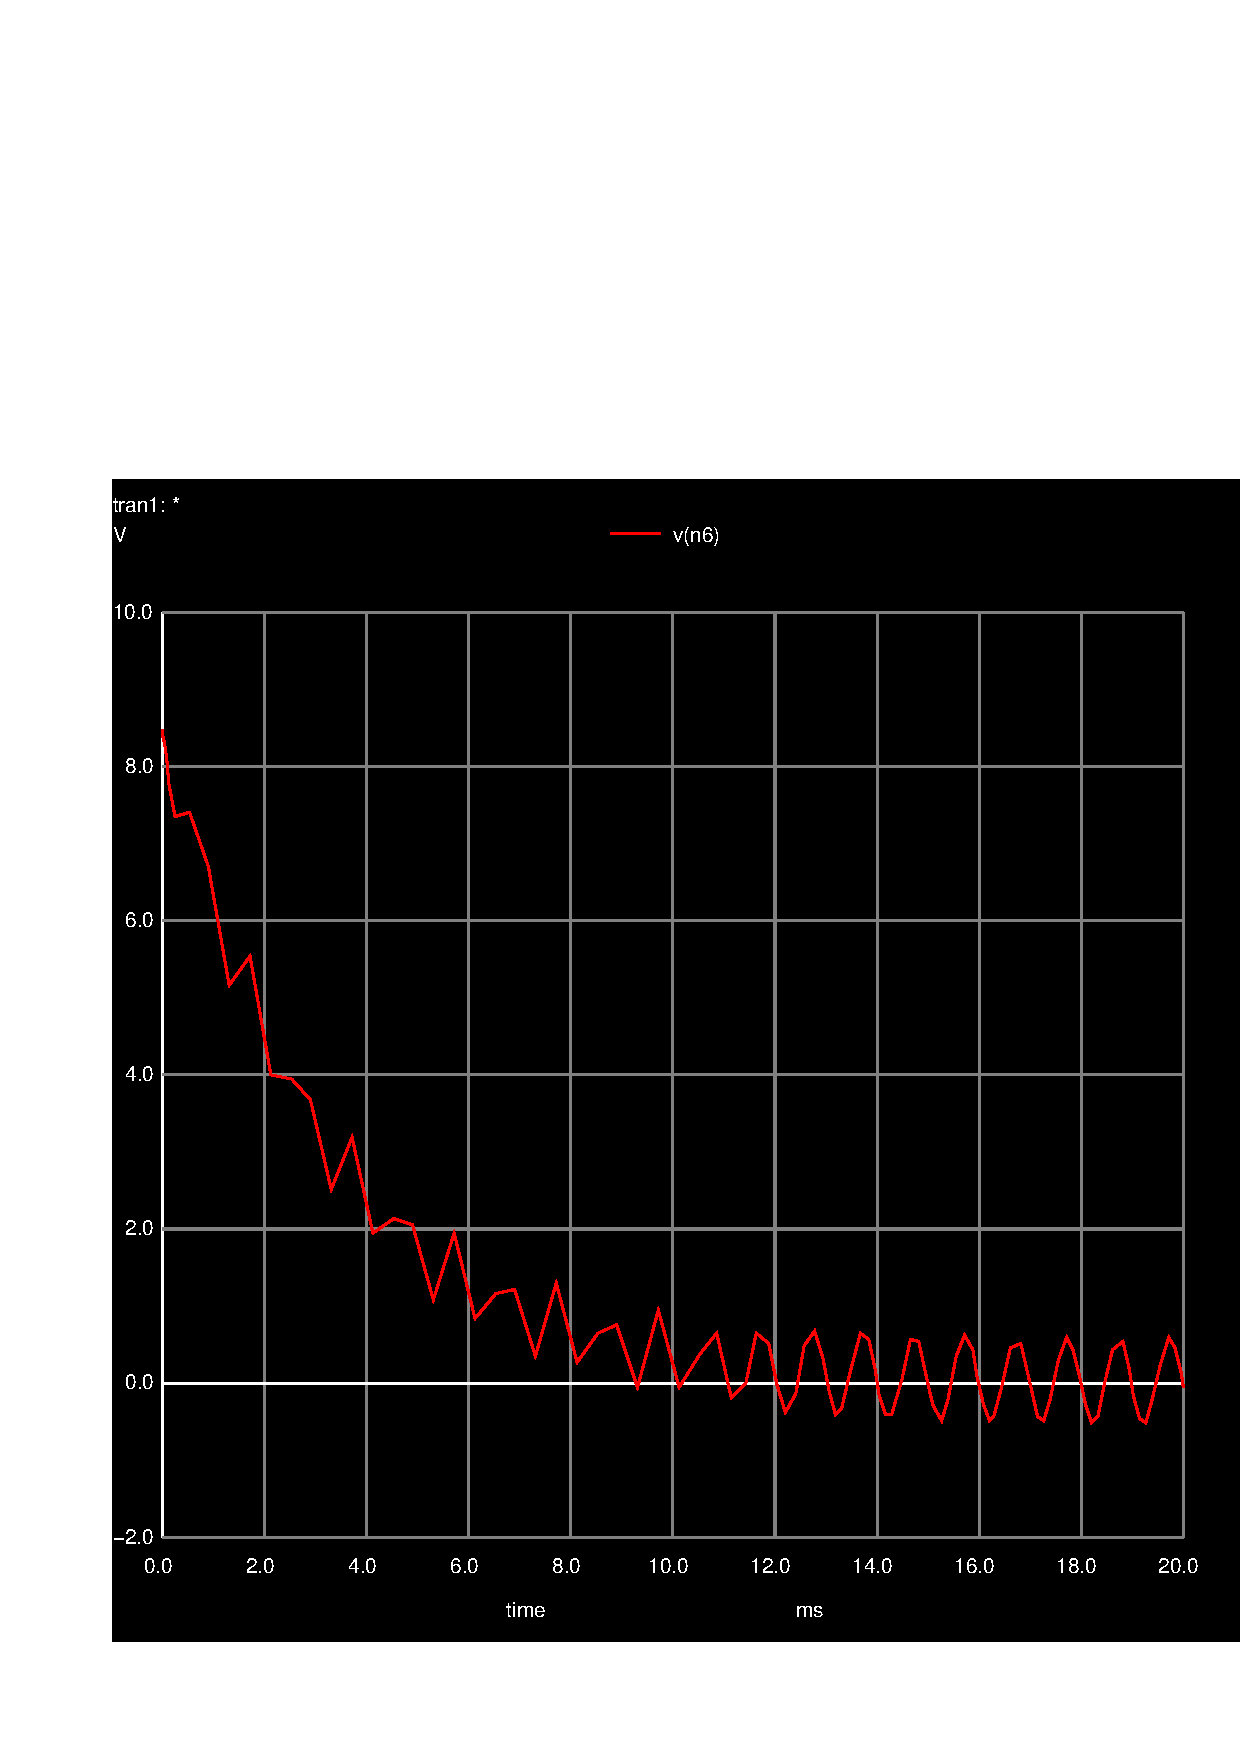
\includegraphics[width=\linewidth]{../sim/transient4r.pdf}
      \caption{Simulation Question 4}
    \endminipage\hfill
\end{figure}

\begin{figure}[H]
    \minipage{0.45\textwidth}
      \includegraphics[width=\linewidth]{../mat/alinea61.pdf}
      \caption{Theoretical Question 6 - Frequency Response}
    \endminipage\hfill
    \minipage{0.45\textwidth}
      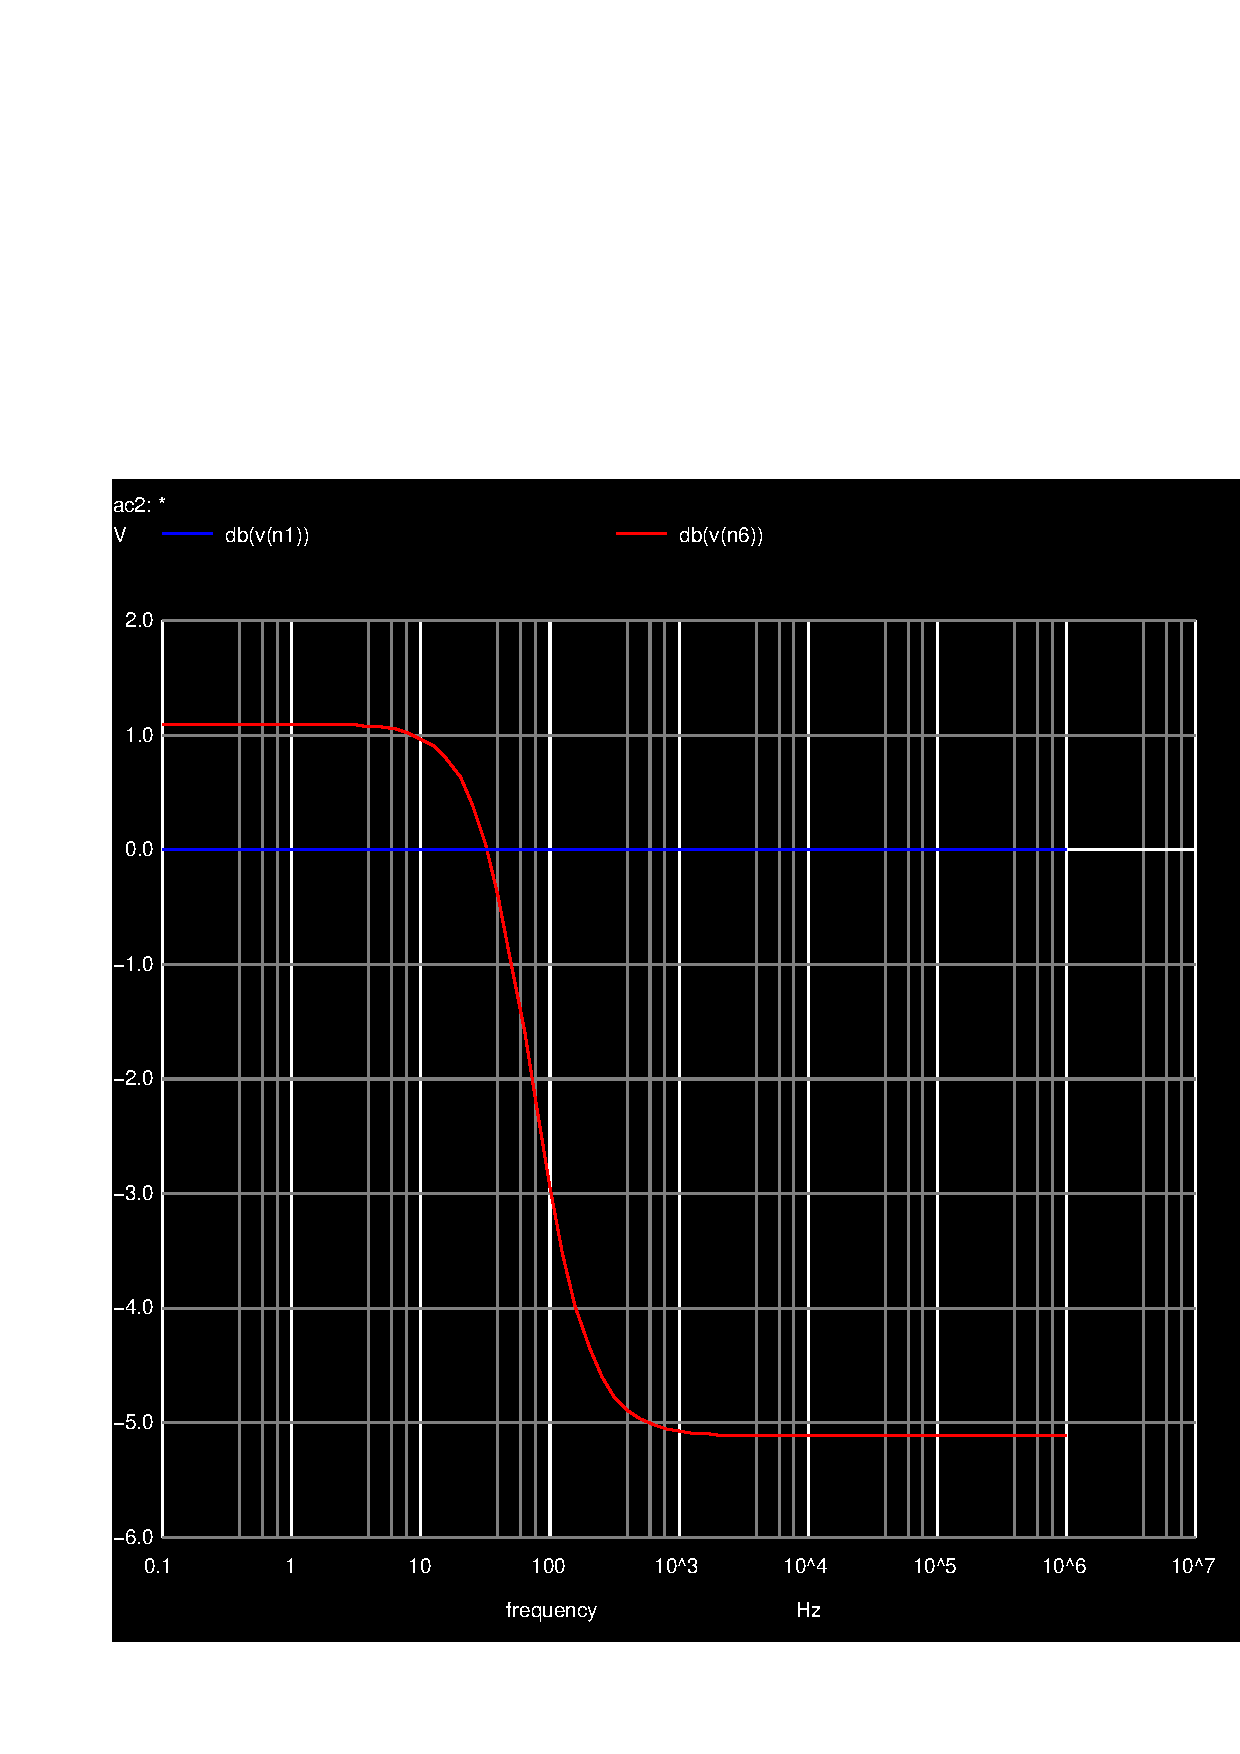
\includegraphics[width=\linewidth]{../sim/fresponse.pdf}
      \caption{Simulation Question 5 - Frequency Response}
    \endminipage\hfill
\end{figure}
